% Options for packages loaded elsewhere
\PassOptionsToPackage{unicode}{hyperref}
\PassOptionsToPackage{hyphens}{url}
\PassOptionsToPackage{dvipsnames,svgnames,x11names}{xcolor}
%
\documentclass[
  9pt,
  letterpaper,
  DIV=11,
  numbers=noendperiod]{scrartcl}

\usepackage{amsmath,amssymb}
\usepackage{setspace}
\usepackage{iftex}
\ifPDFTeX
  \usepackage[T1]{fontenc}
  \usepackage[utf8]{inputenc}
  \usepackage{textcomp} % provide euro and other symbols
\else % if luatex or xetex
  \usepackage{unicode-math}
  \defaultfontfeatures{Scale=MatchLowercase}
  \defaultfontfeatures[\rmfamily]{Ligatures=TeX,Scale=1}
\fi
\usepackage{lmodern}
\ifPDFTeX\else  
    % xetex/luatex font selection
\fi
% Use upquote if available, for straight quotes in verbatim environments
\IfFileExists{upquote.sty}{\usepackage{upquote}}{}
\IfFileExists{microtype.sty}{% use microtype if available
  \usepackage[]{microtype}
  \UseMicrotypeSet[protrusion]{basicmath} % disable protrusion for tt fonts
}{}
\usepackage{xcolor}
\usepackage[lmargin=0.25in,rmargin=0.25in,tmargin=0in,bmargin=0.25in]{geometry}
\setlength{\emergencystretch}{3em} % prevent overfull lines
\setcounter{secnumdepth}{-\maxdimen} % remove section numbering
% Make \paragraph and \subparagraph free-standing
\makeatletter
\ifx\paragraph\undefined\else
  \let\oldparagraph\paragraph
  \renewcommand{\paragraph}{
    \@ifstar
      \xxxParagraphStar
      \xxxParagraphNoStar
  }
  \newcommand{\xxxParagraphStar}[1]{\oldparagraph*{#1}\mbox{}}
  \newcommand{\xxxParagraphNoStar}[1]{\oldparagraph{#1}\mbox{}}
\fi
\ifx\subparagraph\undefined\else
  \let\oldsubparagraph\subparagraph
  \renewcommand{\subparagraph}{
    \@ifstar
      \xxxSubParagraphStar
      \xxxSubParagraphNoStar
  }
  \newcommand{\xxxSubParagraphStar}[1]{\oldsubparagraph*{#1}\mbox{}}
  \newcommand{\xxxSubParagraphNoStar}[1]{\oldsubparagraph{#1}\mbox{}}
\fi
\makeatother


\providecommand{\tightlist}{%
  \setlength{\itemsep}{0pt}\setlength{\parskip}{0pt}}\usepackage{longtable,booktabs,array}
\usepackage{calc} % for calculating minipage widths
% Correct order of tables after \paragraph or \subparagraph
\usepackage{etoolbox}
\makeatletter
\patchcmd\longtable{\par}{\if@noskipsec\mbox{}\fi\par}{}{}
\makeatother
% Allow footnotes in longtable head/foot
\IfFileExists{footnotehyper.sty}{\usepackage{footnotehyper}}{\usepackage{footnote}}
\makesavenoteenv{longtable}
\usepackage{graphicx}
\makeatletter
\def\maxwidth{\ifdim\Gin@nat@width>\linewidth\linewidth\else\Gin@nat@width\fi}
\def\maxheight{\ifdim\Gin@nat@height>\textheight\textheight\else\Gin@nat@height\fi}
\makeatother
% Scale images if necessary, so that they will not overflow the page
% margins by default, and it is still possible to overwrite the defaults
% using explicit options in \includegraphics[width, height, ...]{}
\setkeys{Gin}{width=\maxwidth,height=\maxheight,keepaspectratio}
% Set default figure placement to htbp
\makeatletter
\def\fps@figure{htbp}
\makeatother

\usepackage[pages=some]{background}
% \usepackage{blindtext}
\usepackage[fontsize=8.5pt]{fontsize}

\RedeclareSectionCommand[font=\centering\large]{section}
\RedeclareSectionCommand[
  runin=false,
  afterindent=false,
  font = \normalfont\textbf,
  beforeskip=1pt,
  afterskip=1pt]{subsection}

\setlength{\itemsep}{1pt}
\setlength{\parskip}{0pt}
\setlength{\parsep}{0pt}
\setlength{\labelsep}{0pt}
\setlength{\topsep}{0pt}
\setlength{\parsep}{0pt}
\setlength{\partopsep}{0pt}
\usepackage{fontspec}
\usepackage{multirow}
\usepackage{multicol}
\usepackage{colortbl}
\usepackage{hhline}
\newlength\Oldarrayrulewidth
\newlength\Oldtabcolsep
\usepackage{longtable}
\usepackage{array}
\usepackage{hyperref}
\usepackage{float}
\usepackage{wrapfig}
\KOMAoption{captions}{tableheading}
\makeatletter
\@ifpackageloaded{caption}{}{\usepackage{caption}}
\AtBeginDocument{%
\ifdefined\contentsname
  \renewcommand*\contentsname{Table of contents}
\else
  \newcommand\contentsname{Table of contents}
\fi
\ifdefined\listfigurename
  \renewcommand*\listfigurename{List of Figures}
\else
  \newcommand\listfigurename{List of Figures}
\fi
\ifdefined\listtablename
  \renewcommand*\listtablename{List of Tables}
\else
  \newcommand\listtablename{List of Tables}
\fi
\ifdefined\figurename
  \renewcommand*\figurename{Figure}
\else
  \newcommand\figurename{Figure}
\fi
\ifdefined\tablename
  \renewcommand*\tablename{Table}
\else
  \newcommand\tablename{Table}
\fi
}
\@ifpackageloaded{float}{}{\usepackage{float}}
\floatstyle{ruled}
\@ifundefined{c@chapter}{\newfloat{codelisting}{h}{lop}}{\newfloat{codelisting}{h}{lop}[chapter]}
\floatname{codelisting}{Listing}
\newcommand*\listoflistings{\listof{codelisting}{List of Listings}}
\makeatother
\makeatletter
\makeatother
\makeatletter
\@ifpackageloaded{caption}{}{\usepackage{caption}}
\@ifpackageloaded{subcaption}{}{\usepackage{subcaption}}
\makeatother

\ifLuaTeX
  \usepackage{selnolig}  % disable illegal ligatures
\fi
\usepackage{bookmark}

\IfFileExists{xurl.sty}{\usepackage{xurl}}{} % add URL line breaks if available
\urlstyle{same} % disable monospaced font for URLs
\hypersetup{
  pdftitle={Longfin Inshore Squid () Ecosystem \& Socioeconomic Profile (ESP) Snapshot},
  colorlinks=true,
  linkcolor={blue},
  filecolor={Maroon},
  citecolor={Blue},
  urlcolor={Blue},
  pdfcreator={LaTeX via pandoc}}


\title{Longfin Inshore Squid (\protect\textit{Doryteuthis pealeii})
\linebreak Ecosystem \& Socioeconomic Profile (ESP) Snapshot}
\author{}
\date{}

\begin{document}
\maketitle


\setstretch{1}
\backgroundsetup{
  scale=1,
  angle=0,
  opacity=0,
  contents={
\includegraphics[width=\paperwidth,height=\paperheight]{bg_pg1.jpg}}
 }
\BgThispage

\vspace{-2.0cm}
\section{Spring 2026}

\begin{figure}

\begin{minipage}{0.57\linewidth}

\vspace{0.50cm}
\raggedright
\section{Key Findings from the Life History Working Group}

\subsection{Lifespan and aging}

Growth is estimated to be 1 statolith ring/day, per multiple literature
sources. Participants at the longfin squid summit estimated a maximum
age of 15 months. Literature review supports a lifespan of less than 1
year. Recent (2024) statolith aging indicates maximum ages of 7 months
for females and 8.6 months for males (right) from squid caught in the
fishery.

\vspace{0.25cm}

\subsection{Maturity (from SQUIBS)}

In 2024, most stage 4 squid caught in summer with very little mature
squid caught the rest of the year. Highest numbers of stage 1 squid were
caught in the second half of 2024. Of 912 squid assessed, the dominant
maturity stage in females increases from fall to spring. The highest
percentage of mature male squid were caught in spring and summer. No
stage 4 females and very few stage 1 males were caught.

\vspace{0.25cm}

\subsection{Migration and movement dynamics}

Recent studies suggest the possibility of a winter cohort that hatches
south of Cape Hatteras and subsequently migrates onto the Northeast U.S.
continental shelf. Fishery observations describe a spatial gradient of
1-6 cm mantle length (ML) squid from waters south of Hatteras through
southern New England, with the smallest squid detected further south.
The Gulf Stream and warm core rings may facilitate the recruitment
transport of juvenile squid (Richardson WP), but potential for inputs to
the population from the South and offshore are difficult to quantify.

\vspace{0.25cm}

\subsection{Reproductive dynamics}

Consideration of the hypothesis of a winter cohort spawning south of
Hatteras indicates the presence of multiple cohorts of longfin squid,
with some outside of the traditional Northeast shelf stock area, and
provides evidence of year-round spawning in the stock.

\vspace{0.25cm}

\subsection{Natural mortality}

Although natural mortality is expected to be age-dependent, lack of
accurate age data makes further study difficult. Using the equation
derived by Hamel and Cope (2022), natural mortality for longfin squid
can range from 0.36 (max. age = 15 mo.) to 0.675 (max. age = 8 mo.).
Intraspecific predation impacts natural mortality, but there is no
available data to quantify the amount of mortality this causes.

\vspace{0.25cm}

\vspace{0.50cm}

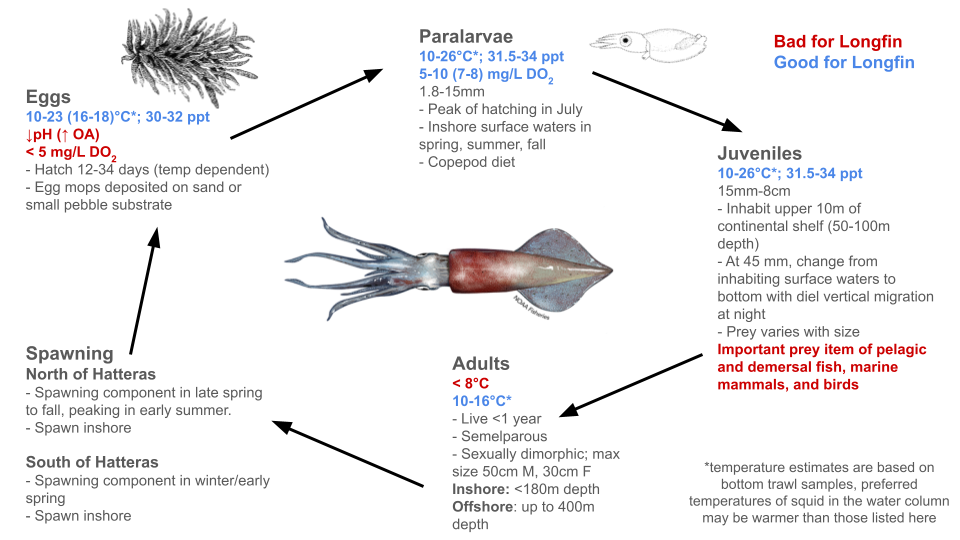
\includegraphics{C:/Users/stephanie.owen/Documents/longfinESP/images/longfin_life_history_0602.png}

\end{minipage}%
%
\begin{minipage}{0.03\linewidth}

\hfill

\end{minipage}%
%
\begin{minipage}{0.40\linewidth}

\vspace{0.50cm}
\section{Age Frequency from SQUIBS}

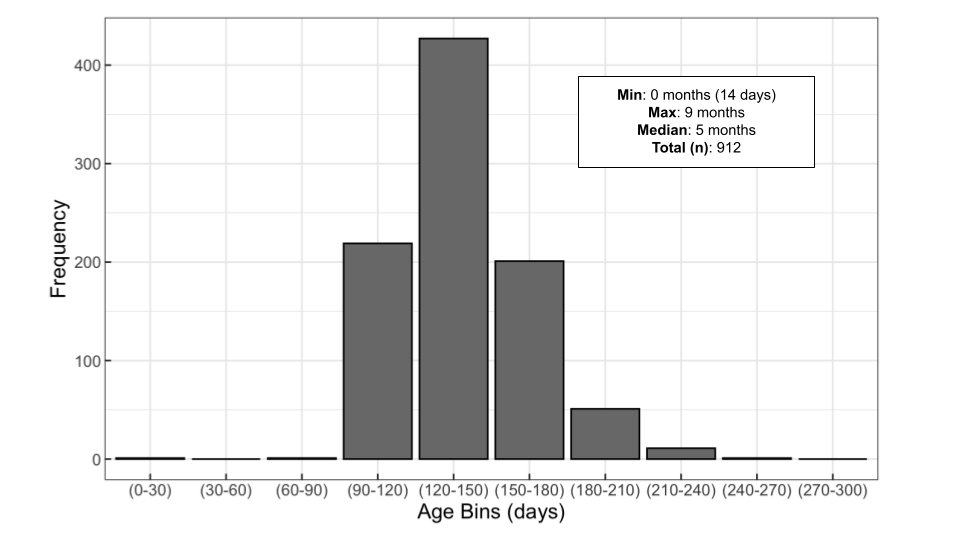
\includegraphics{C:/Users/stephanie.owen/Documents/longfinESP/images/squibs_data.png}

\section{Key Points from the Mid-Atlantic Risk Assessment}

\raggedright

The
\href{https://static1.squarespace.com/static/511cdc7fe4b00307a2628ac6/t/67d45b1680e8654ecaf1b98e/1741970199497/b_Draft+MAB_RiskAssess_2025.pdf}{2025
Mid-Atlantic EAFM Risk Assessment Update} determined that there are
moderate-high risks of :

\begin{itemize}
\tightlist
\item
  Potential and observed distribution shifts of longfin squid
\item
  Not achieving optimum yield due to interactions with non-MAFMC managed
  species
\item
  Regulatory complexity negatively impacting optimum yield due to
  occasional recent changes in regulations and moderate (3-4)
  recreational regulation differences across states
\item
  Not minimizing bycatch and discards to the extent practicable due to
  regular, managed discards and incidental catch and moderate discard
  mortality
\end{itemize}

Risk elements are aspects that may threaten achieving the biological,
economic, or social objectives that the MAFMC desires from a fishery;
risk to achieving optimal yield.

Longfin squid did not score in the ``high'' risk category for any risk
elements in 2025.

\vspace{0.25cm}

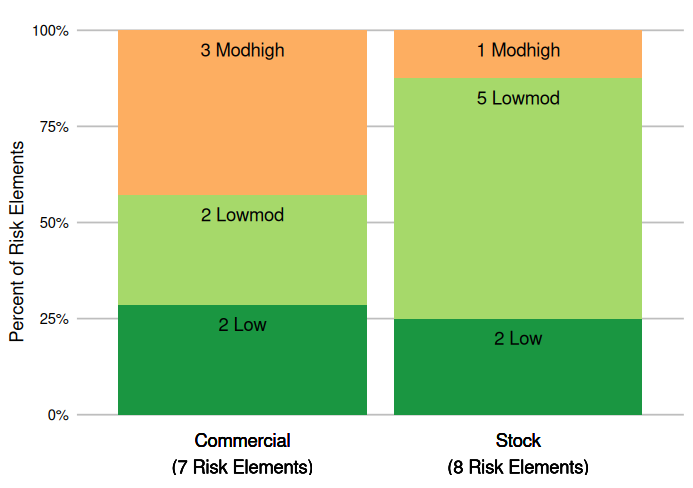
\includegraphics{C:/Users/stephanie.owen/Documents/longfinESP/images/risk_plot_new.png}

\end{minipage}%

\end{figure}%

\newpage

\backgroundsetup{
  contents={
\includegraphics[width=\paperwidth,height=\paperheight]{bg_pg2.jpg}}
  }
\BgThispage

\newgeometry{top=0.25in, left=0.25in, right=0.25in, bottom=0.25in}

\global\setlength{\Oldarrayrulewidth}{\arrayrulewidth}

\global\setlength{\Oldtabcolsep}{\tabcolsep}

\setlength{\tabcolsep}{2pt}

\renewcommand*{\arraystretch}{1.5}



\providecommand{\ascline}[3]{\noalign{\global\arrayrulewidth #1}\arrayrulecolor[HTML]{#2}\cline{#3}}

\begin{longtable*}[c]{|p{0.90in}|p{0.75in}|p{3.00in}|p{3.00in}}



\ascline{0.75pt}{666666}{1-4}

\multicolumn{1}{!{\color[HTML]{666666}\vrule width 0.75pt}>{\centering}m{\dimexpr 0.9in+0\tabcolsep}}{\textcolor[HTML]{000000}{\fontsize{10}{10}\selectfont{\global\setmainfont{Arial}{\textbf{Indicator\ Units}}}}} & \multicolumn{1}{!{\color[HTML]{666666}\vrule width 0.75pt}>{\centering}m{\dimexpr 0.75in+0\tabcolsep}}{\textcolor[HTML]{000000}{\fontsize{10}{10}\selectfont{\global\setmainfont{Arial}{\textbf{Status\ In\ 2024}}}}} & \multicolumn{1}{!{\color[HTML]{666666}\vrule width 0.75pt}>{\centering}m{\dimexpr 3in+0\tabcolsep}}{\textcolor[HTML]{000000}{\fontsize{10}{10}\selectfont{\global\setmainfont{Arial}{\textbf{Implications}}}}} & \multicolumn{1}{!{\color[HTML]{666666}\vrule width 0.75pt}>{\centering}m{\dimexpr 3in+0\tabcolsep}!{\color[HTML]{666666}\vrule width 0.75pt}}{\textcolor[HTML]{000000}{\fontsize{10}{10}\selectfont{\global\setmainfont{Arial}{\textbf{Time\ Series}}}}} \\

\ascline{0.75pt}{666666}{1-4}\endfirsthead 

\ascline{0.75pt}{666666}{1-4}

\multicolumn{1}{!{\color[HTML]{666666}\vrule width 0.75pt}>{\centering}m{\dimexpr 0.9in+0\tabcolsep}}{\textcolor[HTML]{000000}{\fontsize{10}{10}\selectfont{\global\setmainfont{Arial}{\textbf{Indicator\ Units}}}}} & \multicolumn{1}{!{\color[HTML]{666666}\vrule width 0.75pt}>{\centering}m{\dimexpr 0.75in+0\tabcolsep}}{\textcolor[HTML]{000000}{\fontsize{10}{10}\selectfont{\global\setmainfont{Arial}{\textbf{Status\ In\ 2024}}}}} & \multicolumn{1}{!{\color[HTML]{666666}\vrule width 0.75pt}>{\centering}m{\dimexpr 3in+0\tabcolsep}}{\textcolor[HTML]{000000}{\fontsize{10}{10}\selectfont{\global\setmainfont{Arial}{\textbf{Implications}}}}} & \multicolumn{1}{!{\color[HTML]{666666}\vrule width 0.75pt}>{\centering}m{\dimexpr 3in+0\tabcolsep}!{\color[HTML]{666666}\vrule width 0.75pt}}{\textcolor[HTML]{000000}{\fontsize{10}{10}\selectfont{\global\setmainfont{Arial}{\textbf{Time\ Series}}}}} \\

\ascline{0.75pt}{666666}{1-4}\endhead



\multicolumn{1}{!{\color[HTML]{666666}\vrule width 0.75pt}>{\raggedright}m{\dimexpr 0.9in+0\tabcolsep}}{\textcolor[HTML]{000000}{\fontsize{10}{10}\selectfont{\global\setmainfont{Times New Roman}{Commercial\ landings\ (millions\ of\ lbs.)
}}}\textcolor[HTML]{000000}{\fontsize{10}{10}\selectfont{\global\setmainfont{Times New Roman}{\linebreak }}}} & \multicolumn{1}{!{\color[HTML]{666666}\vrule width 0.75pt}>{\raggedright}m{\dimexpr 0.75in+0\tabcolsep}}{\textcolor[HTML]{000000}{\fontsize{10}{10}\selectfont{\global\setmainfont{Times New Roman}{Near\ long\ term\ average}}}} & \multicolumn{1}{!{\color[HTML]{666666}\vrule width 0.75pt}>{\raggedright}m{\dimexpr 3in+0\tabcolsep}}{\textcolor[HTML]{000000}{\fontsize{10}{10}\selectfont{\global\setmainfont{Times New Roman}{Environmental\ dynamics\ vary\ between\ locations/timing\ of\ the\ summer\ and\ winter\ squid\ fisheries.\ An\ increase\ in\ landings\ since\ 2020\ but\ decrease\ in\ number\ of\ vessels\ could\ indicate\ targeted\ trips\ in\ specific\ times\ of\ year\ and\ fishers\ targeting\ other\ species\ when\ longfin\ are\ not\ available.}}}} & \multicolumn{1}{!{\color[HTML]{666666}\vrule width 0.75pt}>{\centering}m{\dimexpr 3in+0\tabcolsep}!{\color[HTML]{666666}\vrule width 0.75pt}}{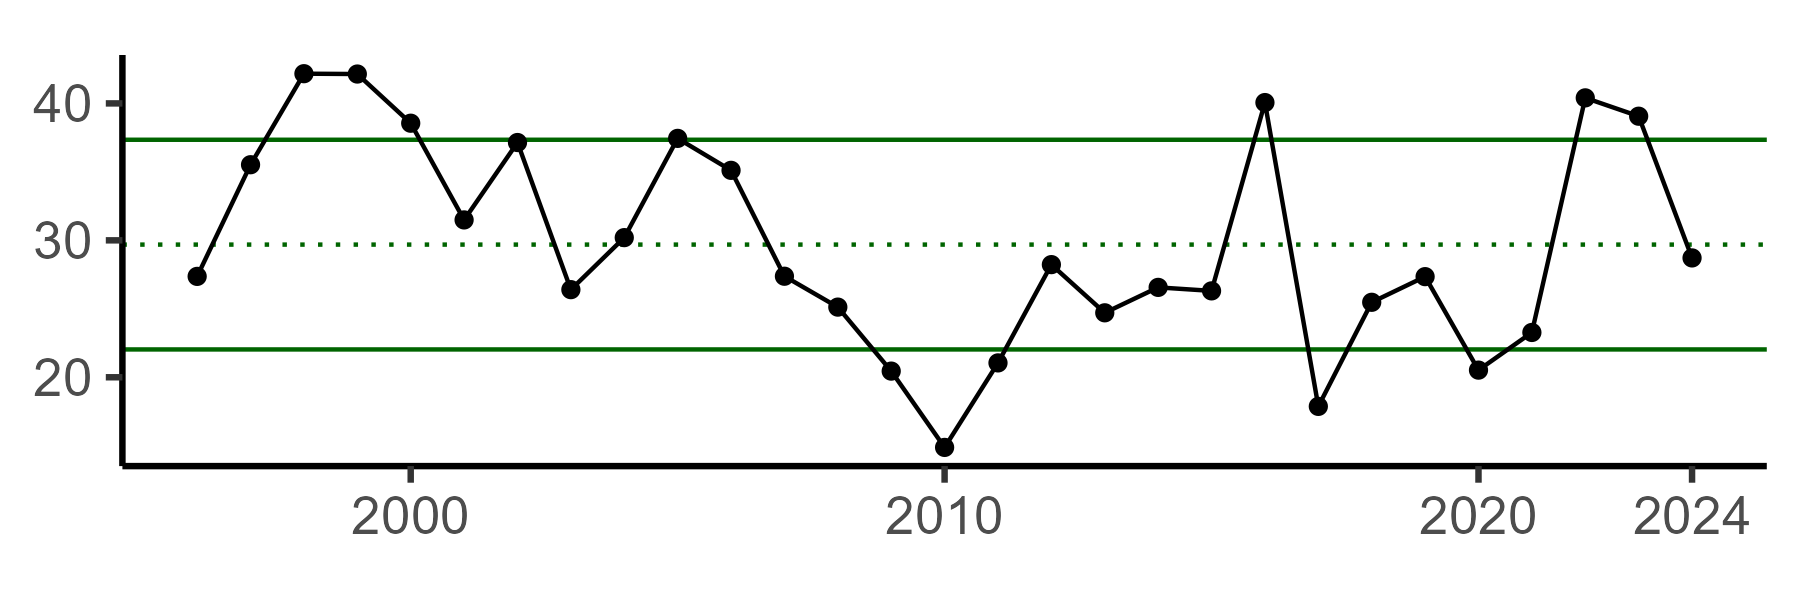
\includegraphics[width=3in, height=1in]{report_card_template_files/figure-pdf/unnamed-chunk-2-1.png}} \\

\ascline{0.75pt}{666666}{1-4}



\multicolumn{1}{!{\color[HTML]{666666}\vrule width 0.75pt}>{\raggedright}m{\dimexpr 0.9in+0\tabcolsep}}{\textcolor[HTML]{000000}{\fontsize{10}{10}\selectfont{\global\setmainfont{Times New Roman}{Number\ of\ commercial\ vessels\ (\#\ \ of\ federally-permitted\ vessels\ landing\ over\ 1lb\ of\ longfin\ squid)}}}} & \multicolumn{1}{!{\color[HTML]{666666}\vrule width 0.75pt}>{\raggedright}m{\dimexpr 0.75in+0\tabcolsep}}{\textcolor[HTML]{000000}{\fontsize{10}{10}\selectfont{\global\setmainfont{Times New Roman}{Below\ long\ term\ average}}}} & \multicolumn{1}{!{\color[HTML]{666666}\vrule width 0.75pt}>{\raggedright}m{\dimexpr 3in+0\tabcolsep}}{\textcolor[HTML]{000000}{\fontsize{10}{10}\selectfont{\global\setmainfont{Times New Roman}{Number\ of\ commercial\ vessels\ has\ been\ steadily\ decreasing\ since\ around\ 2000\ consistent\ with\ decreasing\ fleet\ diversity\ and\ continued\ risk\ to\ fishery\ resilience\ (MAFMC\ FID).\ Permit\ requalification\ in\ 2019\ and\ a\ decrease\ in\ the\ incidental\ limit\ for\ trimester\ 2\ resulted\ in\ fishery\ closures\ in\ 2022\ and\ 2023,\ which\ may\ contribute\ to\ decreased\ participation.}}}} & \multicolumn{1}{!{\color[HTML]{666666}\vrule width 0.75pt}>{\centering}m{\dimexpr 3in+0\tabcolsep}!{\color[HTML]{666666}\vrule width 0.75pt}}{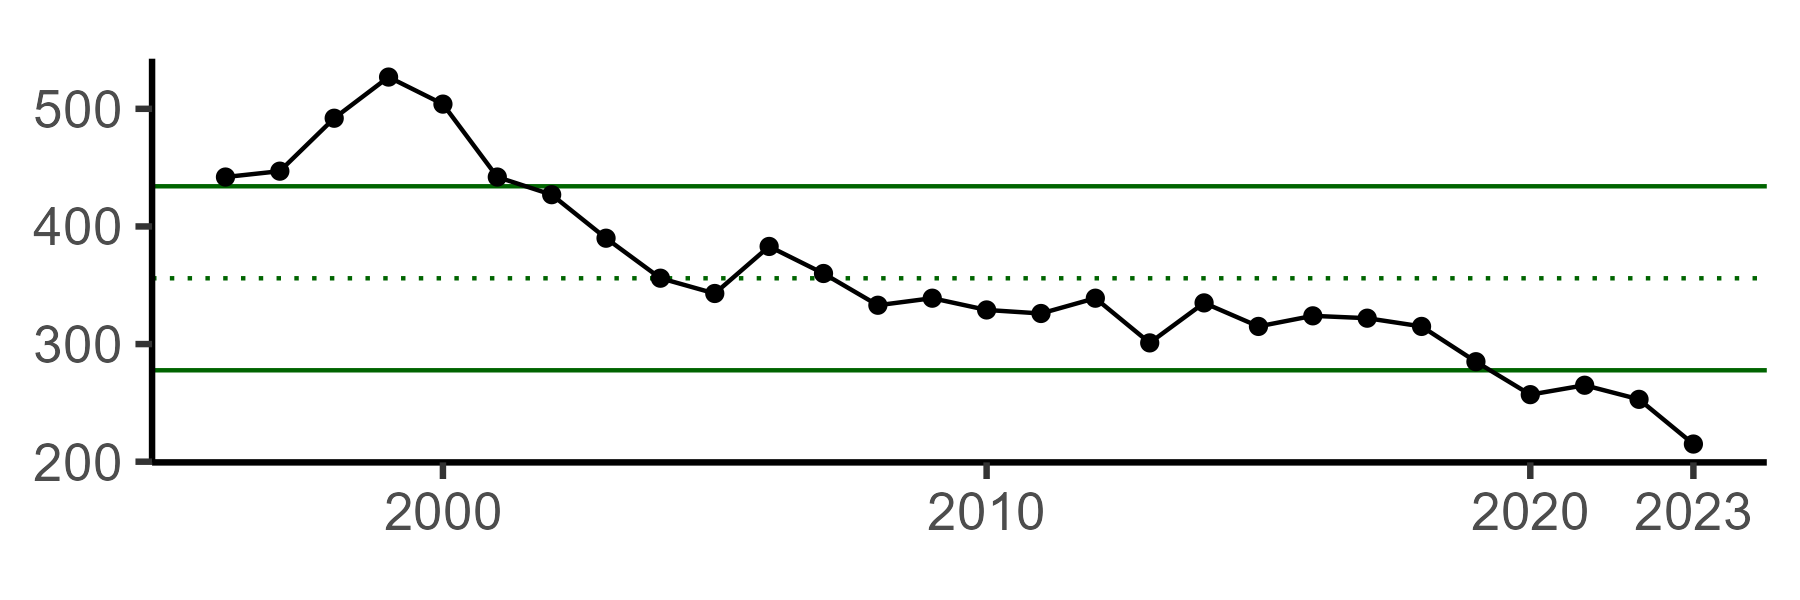
\includegraphics[width=3in, height=1in]{report_card_template_files/figure-pdf/unnamed-chunk-2-2.png}} \\

\ascline{0.75pt}{666666}{1-4}



\multicolumn{1}{!{\color[HTML]{666666}\vrule width 0.75pt}>{\raggedright}m{\dimexpr 0.9in+0\tabcolsep}}{\textcolor[HTML]{000000}{\fontsize{10}{10}\selectfont{\global\setmainfont{Times New Roman}{Commercial\ revenue\ (millions\ 2024\ USD)}}}} & \multicolumn{1}{!{\color[HTML]{666666}\vrule width 0.75pt}>{\raggedright}m{\dimexpr 0.75in+0\tabcolsep}}{\textcolor[HTML]{000000}{\fontsize{10}{10}\selectfont{\global\setmainfont{Times New Roman}{Below\ long\ term\ average}}}} & \multicolumn{1}{!{\color[HTML]{666666}\vrule width 0.75pt}>{\raggedright}m{\dimexpr 3in+0\tabcolsep}}{\textcolor[HTML]{000000}{\fontsize{10}{10}\selectfont{\global\setmainfont{Times New Roman}{Average\ Longfin\ ex-vessel\ prices\ in\ 2024\ increased\ slightly\ from\ 2023\ (+10\%),\ but\ commercial\ revenue\ has\ decreased\ from\ 2023\ which\ is\ most\ likely\ driven\ by\ a\ an\ overall\ decrease\ in\ landings\ by\ 23\%\ (MAFMC\ FID).}}}} & \multicolumn{1}{!{\color[HTML]{666666}\vrule width 0.75pt}>{\centering}m{\dimexpr 3in+0\tabcolsep}!{\color[HTML]{666666}\vrule width 0.75pt}}{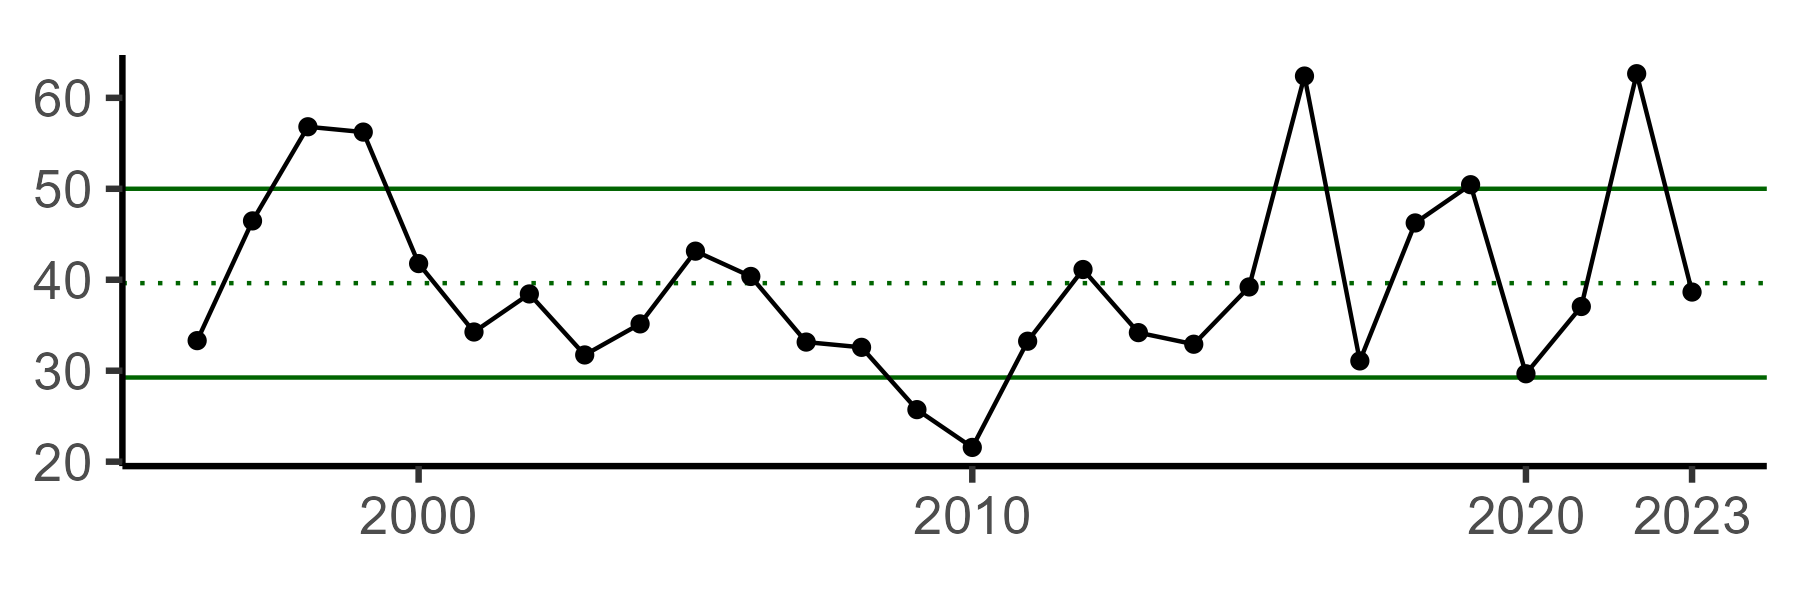
\includegraphics[width=3in, height=1in]{report_card_template_files/figure-pdf/unnamed-chunk-2-3.png}} \\

\ascline{0.75pt}{666666}{1-4}



\multicolumn{1}{!{\color[HTML]{666666}\vrule width 0.75pt}>{\raggedright}m{\dimexpr 0.9in+0\tabcolsep}}{\textcolor[HTML]{000000}{\fontsize{10}{10}\selectfont{\global\setmainfont{Times New Roman}{Western\ Gulf\ Stream\ Index\ (shift\ in\ the\ western\ part\ of\ the\ Gulf\ Stream\ North\ wall:\ mean\ position:\ >0\ =\ more\ northerly,\ <0\ =\ more\ southerly)}}}} & \multicolumn{1}{!{\color[HTML]{666666}\vrule width 0.75pt}>{\raggedright}m{\dimexpr 0.75in+0\tabcolsep}}{\textcolor[HTML]{000000}{\fontsize{10}{10}\selectfont{\global\setmainfont{Times New Roman}{Above\ long\ term\ average}}}} & \multicolumn{1}{!{\color[HTML]{666666}\vrule width 0.75pt}>{\raggedright}m{\dimexpr 3in+0\tabcolsep}}{\textcolor[HTML]{000000}{\fontsize{10}{10}\selectfont{\global\setmainfont{Times New Roman}{Since\ the\ mid-1990s,\ north\ and\ westward\ shifts\ in\ the\ Gulf\ Stream\ have\ resulted\ in\ an\ increase\ in\ warm\ core\ rings\ and\ deep\ water,\ high\ salinity\ heat\ waves.\ The\ position\ of\ the\ Gulf\ Stream\ influences\ seasonal\ temperature\ and\ water\ mass\ mixing\ dynamics\ that\ affect\ longfin\ squid\ habitat\ suitability,\ temperature-dependent\ growth,\ and\ prey\ availability\ (https://noaa-edab.github.io/catalog/gsi.html).}}}} & \multicolumn{1}{!{\color[HTML]{666666}\vrule width 0.75pt}>{\centering}m{\dimexpr 3in+0\tabcolsep}!{\color[HTML]{666666}\vrule width 0.75pt}}{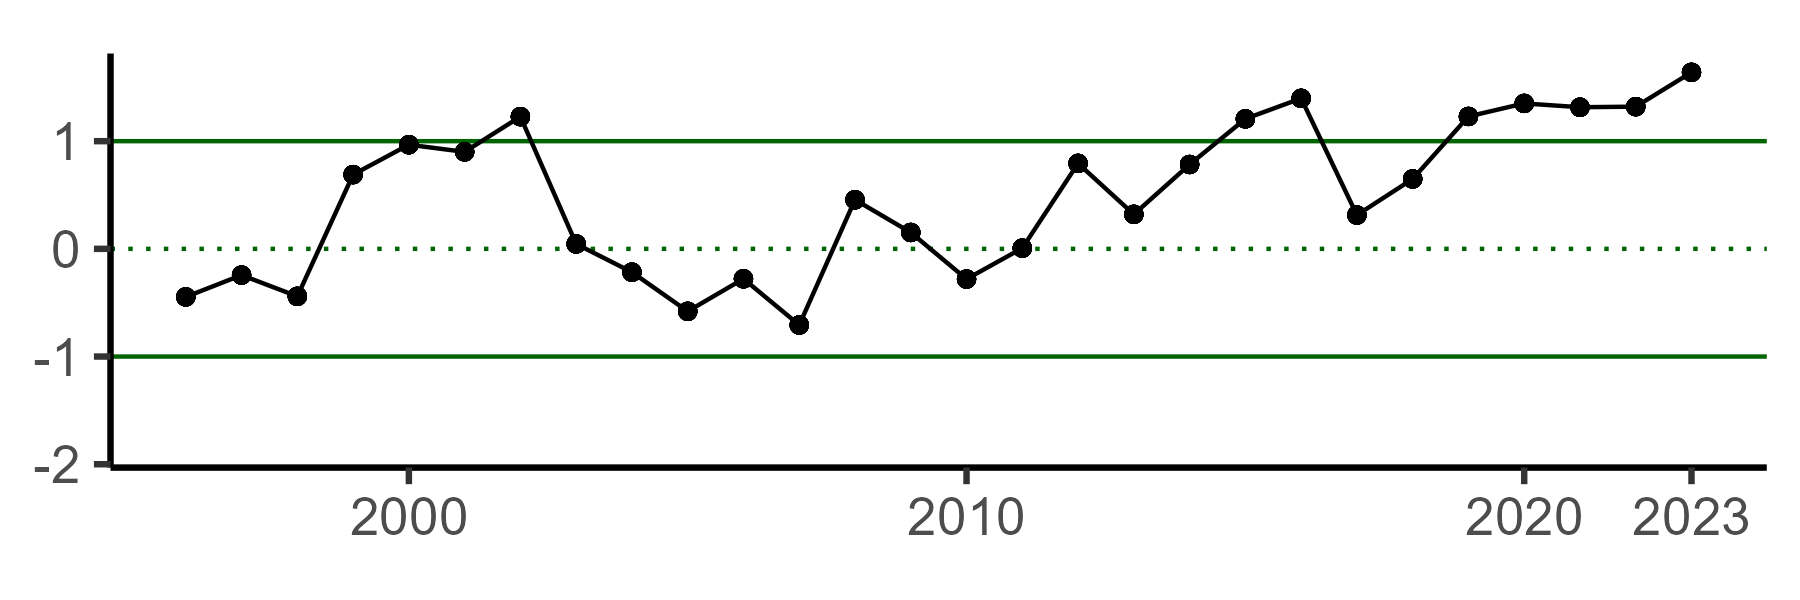
\includegraphics[width=3in, height=1in]{report_card_template_files/figure-pdf/unnamed-chunk-2-4.png}} \\

\ascline{0.75pt}{666666}{1-4}



\multicolumn{1}{!{\color[HTML]{666666}\vrule width 0.75pt}>{\raggedright}m{\dimexpr 0.9in+0\tabcolsep}}{\textcolor[HTML]{000000}{\fontsize{10}{10}\selectfont{\global\setmainfont{Times New Roman}{Bottom\ temperature\ in\ MAB\ and\ SNE(°C)}}}} & \multicolumn{1}{!{\color[HTML]{666666}\vrule width 0.75pt}>{\raggedright}m{\dimexpr 0.75in+0\tabcolsep}}{\textcolor[HTML]{000000}{\fontsize{10}{10}\selectfont{\global\setmainfont{Times New Roman}{Above\ long\ term\ average\ (Fall);\ near\ long\ term\ average\ (Spring)}}}} & \multicolumn{1}{!{\color[HTML]{666666}\vrule width 0.75pt}>{\raggedright}m{\dimexpr 3in+0\tabcolsep}}{\textcolor[HTML]{000000}{\fontsize{10}{10}\selectfont{\global\setmainfont{Times New Roman}{Inshore\ temperature\ thresholds\ (around\ 14°C)\ initiate\ migration\ of\ squid\ from\ offshore\ overwintering\ habitats.\ Longfin\ squid\ seasonal\ distribution\ and\ growth\ rates\ are\ likely\ temperature\ dependent,\ avoiding\ water\ <8°C.\ Stronger\ and/or\ more\ persistent\ Mid-Atlantic\ Cold\ Pool\ conditions\ (not\ shown)\ may\ limit\ habitat\ availability\ (https://noaa-edab.github.io/catalog/cold\_pool.html).}}}} & \multicolumn{1}{!{\color[HTML]{666666}\vrule width 0.75pt}>{\centering}m{\dimexpr 3in+0\tabcolsep}!{\color[HTML]{666666}\vrule width 0.75pt}}{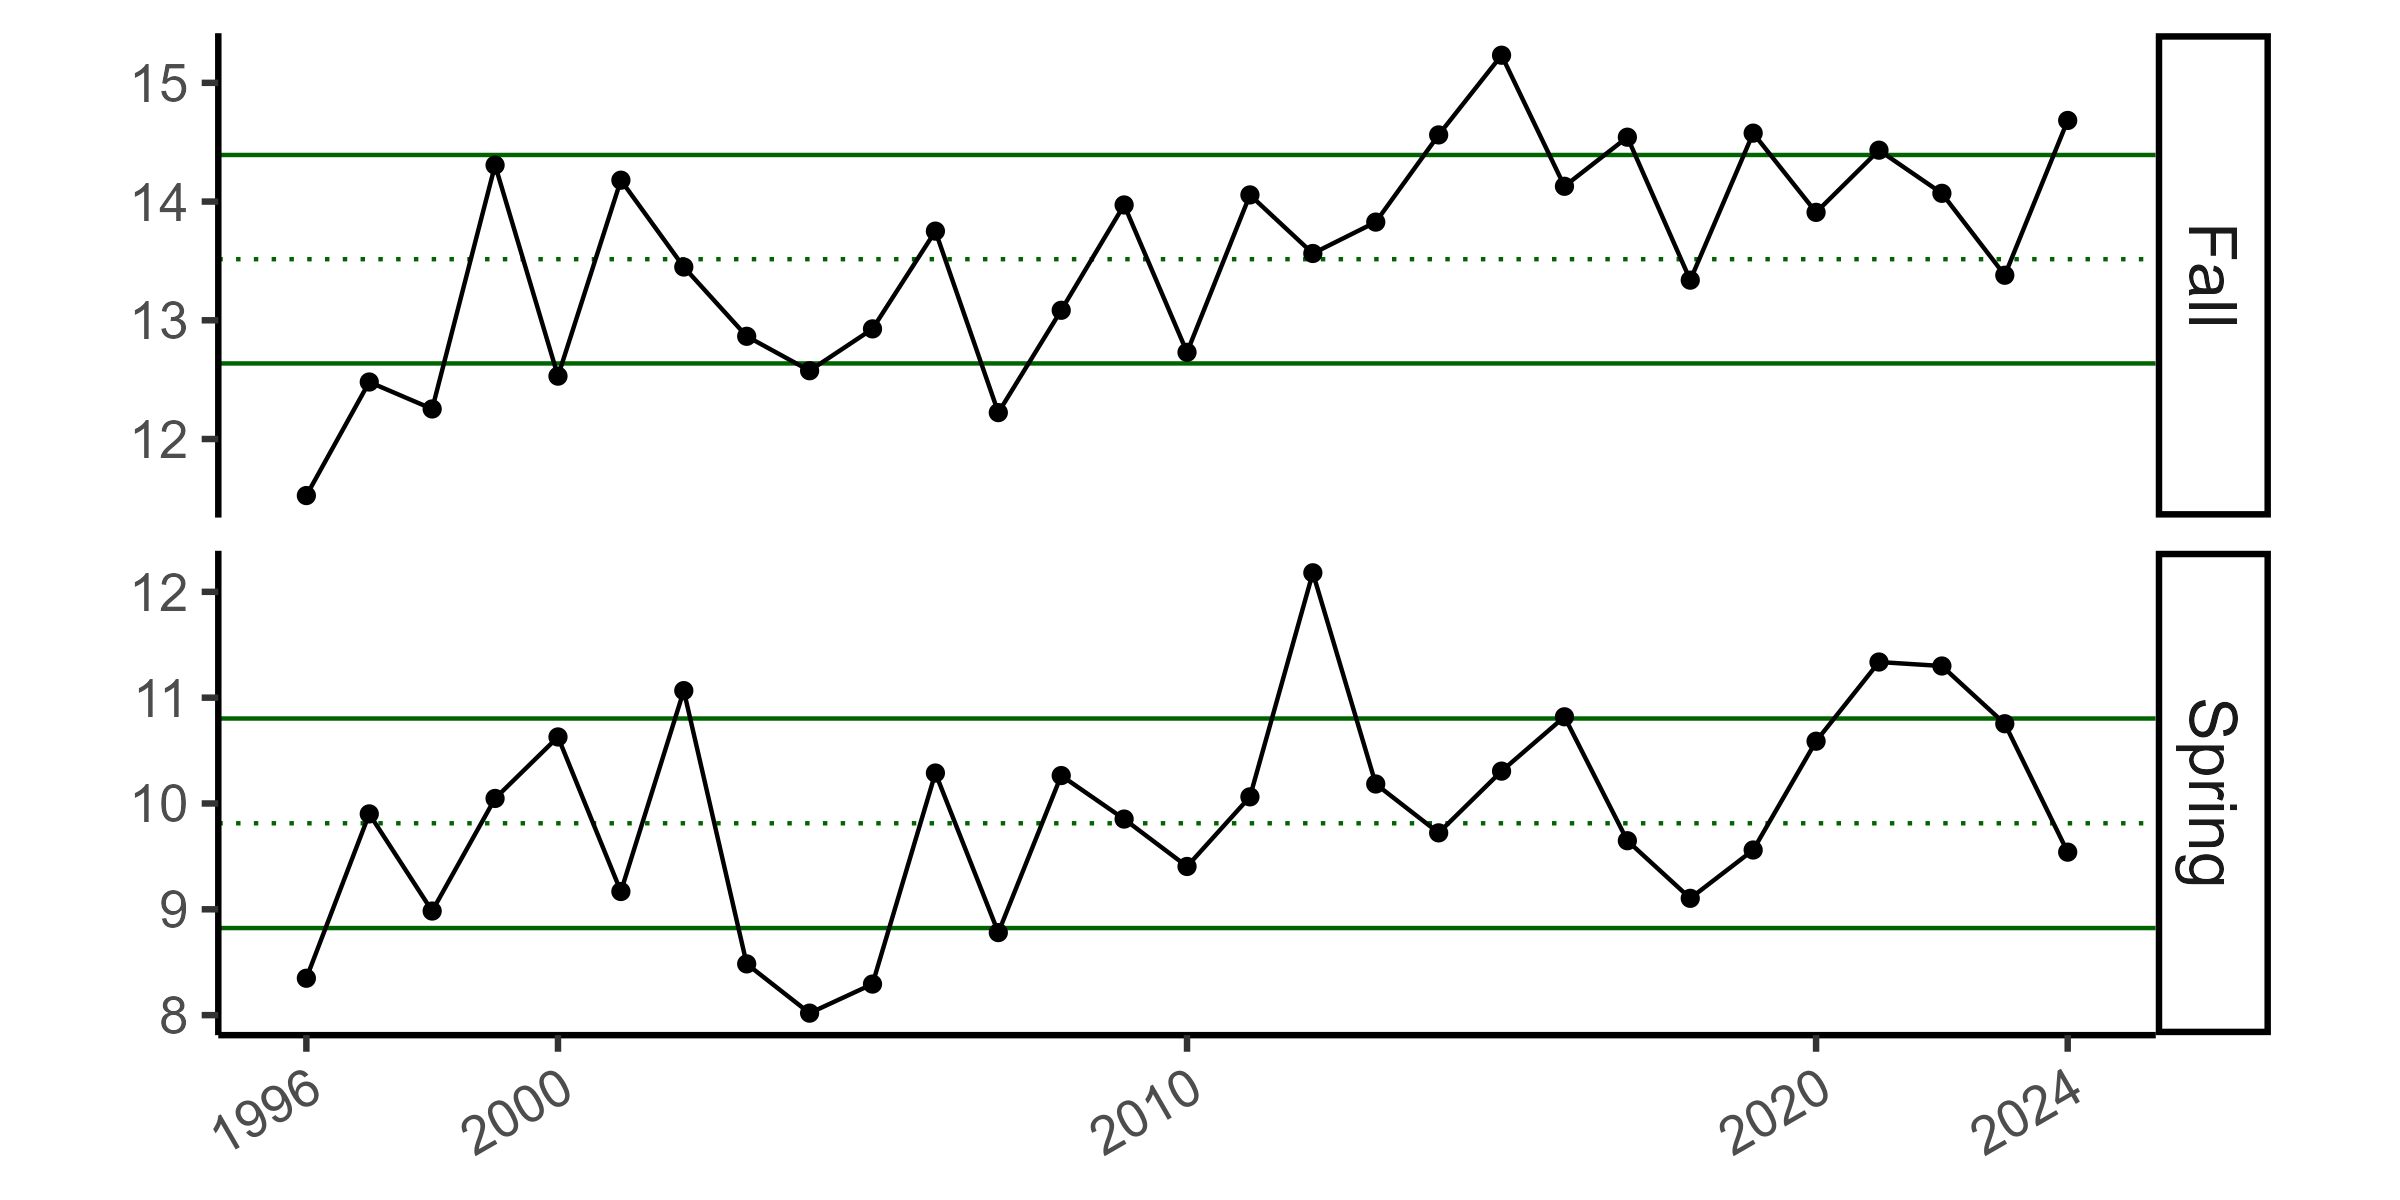
\includegraphics[width=3in, height=1.5in]{report_card_template_files/figure-pdf/unnamed-chunk-2-5.png}} \\

\ascline{0.75pt}{666666}{1-4}



\end{longtable*}



\arrayrulecolor[HTML]{000000}

\global\setlength{\arrayrulewidth}{\Oldarrayrulewidth}

\global\setlength{\tabcolsep}{\Oldtabcolsep}

\renewcommand*{\arraystretch}{1}

\section{Research Recommendations}

\raggedright

-Expand ecosystem and socioeconomic indicator selection relevant to
longfin squid stock dynamics. Potential ecosystem indicators include
bottom salinity, sea surface temperature, warm core rings, marine
heatwaves, storminess index, indices of food availability, and other
oceanographic indicators relevant to shelf/slope dynamics. Potential
socioeconomic indicators include fuel price, quotas, and ex-vessel
price.

\vspace{0.25cm}

-Analyze indicators against longfin squid metrics, such as a
standardized CPUE index.

\vspace{0.25cm}

-Estimate availability of longfin squid stock to fishery independent
surveys and fishery. Through a seasonal habitat suitability
model/species distribution model.

\vspace{0.25cm}

-Evaluate ecosystem and socioeconomic influences on longfin squid in
reference to the stock assessment and fisheries management
considerations.

\vspace{2.0cm}

\centering

Please contact \url{nefsc.esp.leads@noaa.gov} with any questions or
comments.




\end{document}
